\chapter{Princip reflektometrie}

Pojmem \acrfull{TDR} je v této práci myšleno měření vlastností jednobranu pomocí měření odrazů budicího signálu v časové oblasti. Budicím signálem je myšlen obecně jakýkoli kauzální signál. Tento budicí signál je elektricky zaveden do měřeného objektu, načež se měří odezva tohoto systému v čase.
Pokud bychom označili budicí signál jako $x(t)$, měřený signál jako $y(t)$ a impulsní odezvu systému jako $h(t)$, pak pro kauzální lineární časově invariantní systém platí:
\begin{equation}
y(t)=x(t) \ast h(t).
\end{equation}
Cílem takového zařízení je ze známých $x(t)$ a $y(t)$ spočítat nebo odhadnout $h(t)$. Za předpokladu, že měřený systém je elektrické vedení, na kterém se nachází čistě reálný impedanční profil, může odezva vypadat podobně jako na obr. \ref{simpleresponse}, tato impulzní odezva se dá vcelku jednoduše analyzovat \cite{broadbandreflectometry}.

\begin{figure}[htbp]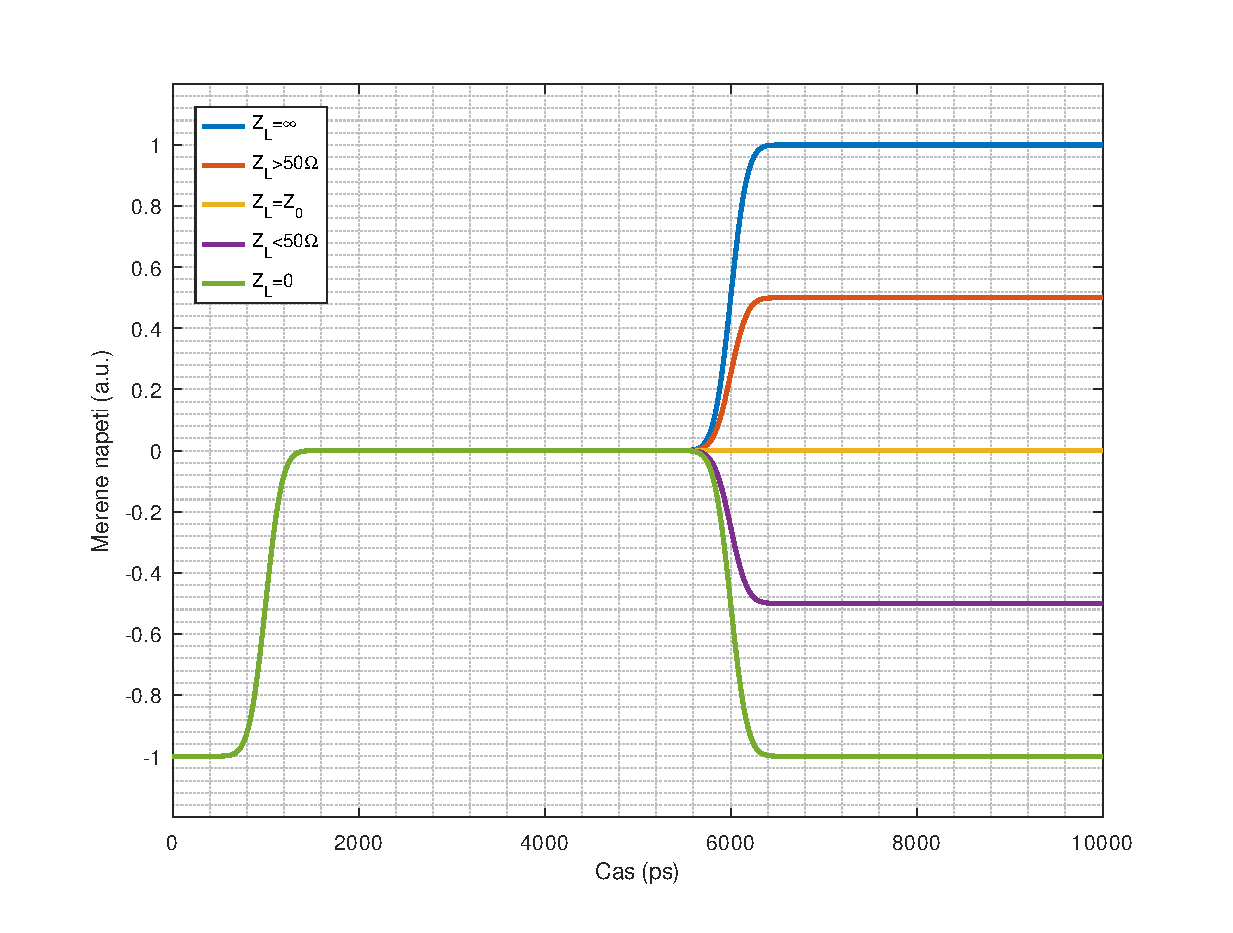
\includegraphics[width=\textwidth,keepaspectratio]{images/onereflectionsample.eps}\caption{Znázornění jednoho odrazu na vedení.}\label{simpleresponse}\end{figure}

Postupně je možné analyzovat tuto impulzní odezvu tak, že se postupuje od okamžiku budicího signálu, až je nalezen první odraz. Z tohoto odrazu a známého budicího signálu je možné spočítat koeficient odrazu \gls{gama} a prostupu \gls{transmise} v daném místě. Dále postupuje jen množství energie definované koeficientem prostupu a energií obsažené v budicím signálu. Při znalosti této energie, koeficientu odrazu dalšího bodu, kde nastává odraz a koeficientu prostupu prvního odrazu (energie odražená od druhé diskontinuity musí opět projít první diskontinuitou). Takto se postupuje až do konce naměřených dat.

Takto jednoduchý postup ovšem zanedbává vliv vícenásobných odrazů. Přesné výsledky dává pouze pro jeden jediný (resp. první) odraz. Čím více diskontinuit na vedení se nachází, tím více se bude nalezené řešení odchylovat od reality. Pro přesnější analýzu je nezbytné, aby byly uvažovány i vícenásobné odrazy. Je možné mezi jednotlivé kroky analýzy impedančního profilu vložit další analytický krok, který zajistí odečtení vlivu vícenásobných odrazů. Tímto krokem je provedení \acrshort{FDTD} simulace s použitím již získaného částečného impedančního profilu, který je virtuálně bezodrazně zakončen. Výsledkem takovéto \acrshort{FDTD} simulace je odezva takovéhoto úseku vedení (jak průběh odraženého signálu, tak i prostupujícího). Nasimulovaný odražený signál je možné odečíst od změřených dat, čímž jsou odstraněny vícenásobné odrazy v již známé části vedení. Dále se pokračuje v analýze tohoto rozdílu měřených a simulovaných dat. Dále se hledá další odraz na vedení a postup se opakuje, dokud není zpracováno celé vedení, nebo dokud energie ve vedení není všechna odražena zpět (platí pro bezeztrátová vedení). Při znalosti fázové rychlosti v daném vedení je možné přepočítat časovou osu na osu prostorovou a odhadnout tedy, kde se nachází diskontinuity.

Dále je možné z těchto odrazů zjišťovat, zda jde o odraz způsobený spojením dvou vedení o rozdílné impedanci (taková diskontinuita se vyznačuje koeficientem odrazu, který se při měření ze dvou stran jeví tak, že má z každé strany koeficient odrazu s jiným znaménkem) nebo o lokální chybu způsobenou například mechanickým poškozením vedení (například navrtaný kabel ve zdi). Taková závada by měla mít z obou stran totožné vlastnosti.

Pro zpracování obecně komplexních koeficientů odrazu (tedy například část vedení, která se chová kapacitně nebo induktivně) by bylo nezbytné vytvořit algoritmus, který by byl schopen rozeznávat v impulsní odezvě nejen čistě reálné odrazy mající v naměřených datech podobu Kroneckerova delta, ale i exponenciální průběhy odpovídající komplexním impedancím, např. na obr. \ref{complexresponse}. Takový algoritmus může být již výrazně náročnější na implementaci, neboť může vyžadovat vícerozměrnou optimalizaci k tomu, aby bylo dosaženo simulací změřené odezvy. Vyvstává také otázka, jak analyzovat, zda jde o přítomnost komplexní impedance na vedení nebo například speciálně zhotovené části vedení, která má spojitý profil impedance, který napodobuje přítomnost komplexní impedance na vedení.

\begin{figure}[htbp]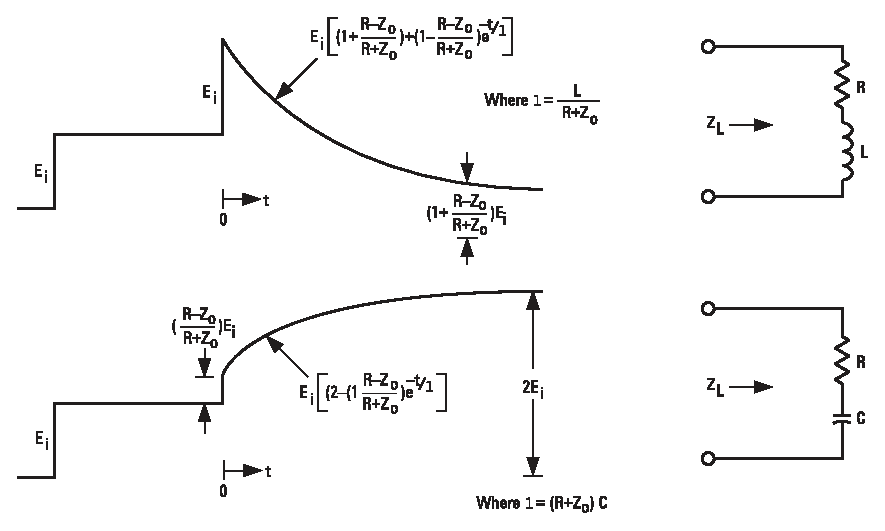
\includegraphics[width=\textwidth,keepaspectratio]{images/samplecomplexresponse.eps}\caption{Příklad odezvy na komplexní impedanci na vedení \cite{broadbandreflectometry}.}\label{complexresponse}\end{figure}

Veškeré tyto úvahy se však týkají převážně bezeztrátových vedení, případně vedení, kde je snadné odhalit ztrátové prvky. Obtížné je například měření útlumu měřeného vedení, neboť samotný útlum vedení nemusí být měřitelný jako odraz. Je-li totiž vedení po celé délce homogenní, nevznikají na něm žádné odrazy, avšak vlivem ztrát dielektrika nebo konečnou vodivostí vodičů se část přenášené energie mění na teplo. Další problém je měření části vedení, která se nachází za ideálním útlumovým článkem nebo nějakým prvkem, který transformuje impedanci. Teoreticky není možné odhalit útlumový článek, pokud není možné různými způsoby zakončit vedení, aby byl odhalen vliv zakončení vedení na celkovou odezvu. I při takovém postupu však není možné určit, kde přesně se takový prvek nachází, protože na něm nevzniká žádný odraz, kterým by bylo možné zjistit jeho polohu. 

Vzhledem ke značné složitosti této analýzy je zpravidla na reflektometrech a kabelových analyzátorech přítomna pouze funkce detekce první diskontinuity, její polohy a charakteru (zkrat, rozpojení, obecně jiná impedance) \cite{CT-100Bmanual} .

Dalším tématem je měření aktivních prvků, neboť v takovém případě je možné dosáhnout koeficientu odrazu s velikostí větší než 1. V takovém případě je možné analýzou pouze zjistit přítomnost aktivního prvku a jeho odezvu, pro zjištění vlastností takového prvku (například vytvoření modelu tranzistoru) je nezbytné znát vnitřní model takového prvku, což již není úlohou reflektometru. Obecně také může být obtížné analyzovat vedení, na kterém se může nacházet nějaký nelineární prvek (takovým případem může být i například přítomnost vlhkosti ve vedení, která změní impedanci vedení, ovšem nad přibližně 3\,GHz kvůli dielektrické relaxaci přestane mít vliv \cite{relaxationspectroscopy}).

Závěrem této části práce může být tedy konstatování, že je jednoduché odhalit první diskontinuitu (nebo největší, jsou-li ostatní dostatečně malé). Obtížnější je charakterizovat ji, má-li komplexní imepdanci. Mnohem obtížnější je analýza celého vedení, v případě uvažování obecně komplexní impedance může být nemožné získat jednoznačnou analýzu takového vedení, protože může být způsobena jak komplexní impedancí na vedení, tak i několika blízkými závadami na vedení. Přítomnost nelinearit na vedení může zcela znemožnit jakoukoli analýzu nebo způsobit celkovou nesprávnost takové analýzy.

V dalších kapitolách budou rozebrány jednotlivé stavební bloky nezbytné pro konstrukci \acrshort{TDR} a možnosti jejich implementace s přihlédnutím k jednoduchosti fyzické implementace a možností následného zpracování naměřených dat.